\documentclass[hidelinks,12pt,openany,letterpaper,pagesize]{scrbook}

%\usepackage[ansinew]{inputenc}
\usepackage{xltxtra}
\usepackage[english]{babel}
\usepackage{fancyhdr}
\usepackage{epsfig}
\usepackage{epic}
\usepackage{eepic}
\usepackage{amsmath}
\usepackage{threeparttable}
\usepackage{amscd}
\usepackage{here}
\usepackage{graphicx}
\usepackage{lscape}
\usepackage{tabularx}
\usepackage{subfigure}
\usepackage{longtable}


\usepackage{multicol}
\usepackage[colorinlistoftodos]{todonotes}
\usepackage{subfigure} 
\usepackage{anysize} 
\usepackage{caption}
\usepackage{dsfont}
\usepackage[export]{adjustbox}

\usepackage[nottoc,numbib]{tocbibind} 

\usepackage{xcolor}

\usepackage[colorlinks=true, linkcolor=black, citecolor=black, urlcolor=black]{hyperref}

\DeclareMathAlphabet{\mathpzc}{OT1}{pzc}{m}{it}



% Tipografía de la Universidad Nacional de Colombia 2016.
% http://identidad.unal.edu.co/guia-de-identidad-visual/

\setmainfont[
Path = Ancizar/,
Extension       = .otf,
UprightFont     = *-Light,
BoldFont        = *-Semibold,
ItalicFont      = *-LightItalic,
BoldItalicFont  = *-SemiboldItalic,
%SlantedFont     = *-⟨font name⟩,
%BoldSlantedFont = *-⟨font name⟩,
%SmallCapsFont   = *-⟨font name⟩,
]{AncizarSerif}

\setsansfont[
Path = Ancizar/,
Extension       = .otf,
UprightFont     = *-Light,
BoldFont        = *-Semibold,
ItalicFont      = *-LightItalic,
BoldItalicFont  = *-SemiboldItalic,
%SlantedFont     = *-⟨font name⟩,
%BoldSlantedFont = *-⟨font name⟩,
%SmallCapsFont   = *-⟨font name⟩,
]{AncizarSerif}

\usepackage{rotating} %Para rotar texto, objetos y tablas seite. No se ve en DVI solo en PS. Seite 328 Hundebuch
                        %se usa junto con \rotate, \sidewidestable ....


\renewcommand{\theequation}{\thechapter-\arabic{equation}}
\renewcommand{\thefigure}{\textbf{\thechapter-\arabic{figure}}}
\renewcommand{\thetable}{\textbf{\thechapter-\arabic{table}}}


\pagestyle{fancyplain}%\addtolength{\headwidth}{\marginparwidth}
\textheight22.5cm \topmargin0cm \textwidth16.5cm
\oddsidemargin0.5cm \evensidemargin-0.5cm%
\renewcommand{\chaptermark}[1]{\markboth{\thechapter\; #1}{}}
\renewcommand{\sectionmark}[1]{\markright{\thesection\; #1}}
\lhead[\fancyplain{}{\thepage}]{\fancyplain{}{\rightmark}}
\rhead[\fancyplain{}{\leftmark}]{\fancyplain{}{\thepage}}
\fancyfoot{}
\thispagestyle{fancy}%


\addtolength{\headwidth}{0cm}
\unitlength1mm %Define la unidad LE para Figuras
%\mathindent0cm %Define la distancia de las formulas al texto,  fleqn las descentra
\marginparwidth0cm
\parindent0cm %Define la distancia de la primera linea de un parrafo a la margen

%Para tablas,  redefine el backschlash en tablas donde se define la posici\'{o}n del texto en las
%casillas (con \centering \raggedright o \raggedleft)
\newcommand{\PreserveBackslash}[1]{\let\temp=\\#1\let\\=\temp}
\let\PBS=\PreserveBackslash

%Espacio entre lineas
\renewcommand{\baselinestretch}{1.1}

%Neuer Befehl f\"{u}r die Tabelle Eigenschaften der Aktivkohlen
\newcommand{\arr}[1]{\raisebox{1.5ex}[0cm][0cm]{#1}}

%Neue Kommandos
\usepackage{Befehle}


%Trennungsliste
\hyphenation {Reaktor-ab-me-ssun-gen Gas-zu-sa-mmen-set-zung
Raum-gesch-win-dig-keit Durch-fluss Stick-stoff-gemisch
Ad-sorp-tions-tem-pe-ra-tur Klein-schmidt
Kohlen-stoff-Mole-kular-siebe Py-rolysat-aus-beu-te
Trans-port-vor-gan-ge}
%\includeonly{Kap1/Kap1,Kap2/Kap2}
\begin{document}
\pagenumbering{roman}
%\newpage
%\setcounter{page}{1}
\begin{center}
\begin{figure}
\centering%

\includegraphics[width=6.5cm]{HojaTitulo/EscudoUN}
\end{figure}
\thispagestyle{empty} \vspace*{1.0cm} \textbf{\huge
Choosing Adequate Speech Presence Probability Method for Enhanced Multichannel Background Noise Reduction Algorithms}\\[4.0cm]
\Large\textbf{Iván Darío Arévalo Gutiérrez}\\[4.0cm]
\small Universidad Nacional de Colombia\\
Facultad de Ingeniería, Departamento de Ingeniería Eléctrica y Electrónica.\\
Bogotá, Colombia\\
2017\\
\end{center}

\newpage{\pagestyle{empty}\cleardoublepage}

\newpage
\begin{center}
\thispagestyle{empty} \vspace*{0cm} \textbf{\huge
Choosing Adequate Speech Presence Probability Method for Enhanced Multichannel Background Noise Reduction Algorithms}\\[3.0cm]
\Large\textbf{Iván Darío Arévalo Gutiérrez}\\[3.0cm]
\small Trabajo de grado presentado como requisito parcial para optar al
t\'{\i}tulo de:\\
\textbf{Pregrado en Ingeniería Electrónica}\\[2.5cm]
Director:\\
Jan Bacca Rodríguez Ph.D.\\[4.5cm]

Universidad Nacional de Colombia\\
Facultad de Ingeniería, Departamento de Ingeniería Eléctrica y Electrónica.\\
Bogotá, Colombia\\
2017\\
\end{center}

\newpage{\pagestyle{empty}\cleardoublepage}

\newpage
\thispagestyle{empty} \textbf{}\normalsize
\\\\\\%

\begin{flushright}
\begin{minipage}{8cm}
    \noindent
        \small
        \textit{"The voice of beauty speaks softly; it creeps only into the most fully awakened souls”} \\
- Friedrich Nietzsche
\end{minipage}
\end{flushright}

\newpage
\thispagestyle{empty} \textbf{}\normalsize
\\\\\\%
\textbf{\LARGE Acknowledgment}
\addcontentsline{toc}{chapter}{Acknowledgment}\\\\

I want to give special thanks to all the pedagogic staff at the Universidad Nacional de Colombia, who guided me to achieve my dreams.\\

Also, I would like to thank all the team of the Universidad de Colombia Radio (UN Radio), who gave their time and knowledge to help me recording an appropriated data base for this project.\\  

Finally I would also like to thank all my family and my friends, who always believed in me and have given me all the support I need to continue.\\

\newpage{\pagestyle{empty}\cleardoublepage}

\newpage


\textbf{\LARGE Abstract}\\\\

There are several voice communication systems that are used nowadays which are capable of maintain voice calls between two users in real time. Telephones are widely used all around the world in an unlimited kind of situations. All of these situations expose the microphone (or microphones) of the phones to different and unpredictable noises, as street noise, sea noise, rain noise, wind noise, unwanted voices, car motors, etc. As microphones capture all the sounds around it, including the wanted voice and the unwanted noises, it is necessary to implement digital real time filters capable of attenuate as much as possible all the surrounding noises. \\

It exists a large quantity of noise reduction methods that have been used in the calling algorithms of phones. Even if these methods have had, in general, a good performance, there is still a research being done in this area in order to improve the current results. Because of this, the multichannel methods were created (using multiple microphones) as well as new algorithms that pretend to have a better noise reduction than the single channel methods. Most of these methods require a speech presence probability (SPP) method to achieve the noise reduction.\\

The following document presents a research about different SPP methods as well as a comparison between these. This includes an explanation on how theses algorithm work, a Matlab implementation using real voice and noise recordings and objective tests of the filter. \\



\textbf{\small Key Words: Noise suppression, Speech processing, Speech enhancement, Adaptive signal processing, Active filters, Digital filters, Noise, Low-frequency noise, Noise cancellation, Signal to noise ratio}.\\




\renewcommand{\tablename}{\textbf{Table}}
\renewcommand{\figurename}{\textbf{Figure}}
\renewcommand{\listtablename}{Lista de Tablas}
\renewcommand{\listfigurename}{Lista de Figuras}
\renewcommand{\contentsname}{Contents}


%\newcommand{\clearemptydoublepage}{\newpage{\pagestyle{empty}\cleardoublepage}}
\tableofcontents
%\chapter*{Lista de s\'{\i}mbolos}
\addcontentsline{toc}{chapter}{\numberline{}Lista de s\'{\i}mbolos}
Esta secci\'{o}n es opcional, dado que existen disciplinas que no manejan s\'{\i}mbolos y/o abreviaturas.\\

Se incluyen s\'{\i}mbolos generales (con letras latinas y griegas), sub\'{\i}ndices, super\'{\i}ndices y abreviaturas (incluir s\'{o}lo las clases de s\'{\i}mbolos que se utilicen). Cada una de estas listas debe estar ubicada en orden alfab\'{e}tico de acuerdo con la primera letra del s\'{\i}mbolo.
\section*{S\'{\i}mbolos con letras latinas}
 \label{simbolos}
 \renewcommand{\arraystretch}{1.3}
%\begin{longtable}[l]{*{4}{>{$}l<{$}}p{9cm}}
\begin{longtable}[l]{>{$}l<{$}l>{$}l<{$}>{$}l<{$}}
%\begin{tabular}
\textbf{S\'{\i}mbolo}&\textbf{T\'{e}rmino}&\textbf{Unidad SI}&\textbf{Definici\'{o}n}\\[0.5ex]\hline
\endfirsthead%
\textbf{S\'{\i}mbolo}&\textbf{T\'{e}rmino}&\textbf{Unidad SI}&\textbf{Definici\'{o}n}\\[0.5ex]\hline
\endhead%
      A              &\'{A}rea                                   &\text{m}^{2}                         &\int\int dxdy\\%
      A_{\text{BET}} &\'{A}rea interna del s\'{o}lido                &\frac{\text{m}^{2}}{\text{g}}        &\text{ver DIN ISO 9277}\\%
      A_{\text{g}}   &\'{A}rea transversal de la fase gaseosa    &\text{m}^{2}                         &\text{Ec...}\\%
      A_{\text{s}}   &\'{A}rea transversal de la carga a granel  &\text{m}^{2}                         &\text{Ec...}\\%
      a              &Coeficiente                            &1                                    &\text{Ec...}\\%
      a              &Contenido de ceniza                    &1                                    &\frac{m_{\text{ceniza}}}{m_{\text{bm,0}}}\\%
      c              &Contenido de carbono                   &1                                    &\frac{m_{\text{C}}}{m}\\%
      c              &Longitud de la cuerda                  &\text{m}                             &\text{Figura...}\\
      c              &Concentraci\'{o}n de la cantidad de materia&\frac{\text{mol}}{\text{m}^{3}}      &\frac{n}{V}\\%
      D              &Di\'{a}metro                               &\text{m}                             &\\%
      E_{\text{A}}   &Energ\'{\i}a de activaci\'{o}n                  &\frac{\text{kJ}}{\text{mol}}         &\text{Ec....}\\%
      F              &Fracci\'{o}n de materia vol\'{a}til            &1                                    &\text{ver DIN 51720}\\%
      Fr             &N\'{u}mero de Froude                       &1                                    &\frac{\omega^{2}R}{g_{\text{0}}}\\%
      \overrightarrow{g}&Aceleraci\'{o}n de la gravedad          &\frac{\text{m}}{\text{s}^{2}}        &\frac{d^{2}\overrightarrow{r}}{dt^{2}}\\%
      H              &Entalp\'{\i}a                               &\text{J}                             &U+PV\\%
      H_{\text{o}}   &Poder calor\'{\i}fico superior              &\frac{\text{MJ}}{\text{kg}}          &\text{ver DIN 51857}\\%
      h              &Contenido de hidr\'{o}geno                 &1                                    &\frac{m_{\text{H}}}{m}\\%
      K              &Coeficiente de equilibrio              &1                                    &\text{Ec...}\\%
      L              &Longitud                               &\text{m}                             &DF\\%
      L              &Longitud del reactor                   &\text{m}                             &\text{Figura...}\\%
      m              &Masa                                   &\text{kg}                            &DF\\%
      \dot{m}        &Flujo de masa                          &\frac{\text{kg}}{\text{s}}           &\frac{m}{t}\\%
      n              &Velocidad de rotaci\'{o}n                  &\frac{\text{1}}{\text{s}}            &\frac{\omega}{2\pi}\\%
      n              &Cantidad de materia                    &\text{mol}                           &DF\\%
      P              &Presi\'{o}n                                &\text{Pa}                            &\frac{\vec{F}\cdot\vec{n}}{A}\\%
      Q              &Calor                                  &\text{kJ}                            &\text{1. $LT$}\\%
      T              &Temperatura                            &\text{K}                             &DF\\%
      t              &Tiempo                                 &\text{s}                             &DF\\%
      x_{\text{i}}   &Fracci\'{o}n de la cantidad de materia     &1                                    &\frac{n_{\text{i}}}{n}\\%
      V              &Volumen                                &\text{m}^{3}                         &\int{dr^{3}}\\%
      \vec{u}        &Velocidad                              &\frac{\text{m}}{\text{s}}            &(\frac{dr}{dt},r\frac{d\upsilon}{dt},\frac{dz}{dt})\\%
      w_{\text{i}}   &Fracci\'{o}n en masa del componente i      &1                                    &\frac{m_{\text{i}}}{m_{\text{0}}}\\%
      w_{\text{w,i}} &Contenido de humedad de la sustancia i &1                                    &\frac{m_{\text{\wasser}}}{m_{\text{i,0}}}\\%
      Z              &Factor de gases reales                 &1                                    &\frac{pv}{RT}\\%
\end{longtable}
\vspace{5ex}
\section*{S\'{\i}mbolos con letras griegas}

\begin{longtable}[l]{>{$}l<{$}l>{$}l<{$}>{$}l<{$}}
\textbf{S\'{\i}mbolo}&\textbf{T\'{e}rmino}&\textbf{Unidad SI}&\textbf{Definici\'{o}n}\\[0.5ex] \hline%
\endfirsthead%
\textbf{S\'{\i}mbolo}&\textbf{T\'{e}rmino}&\textbf{Unidad SI}&\textbf{Definici\'{o}n}\\[0.5ex] \hline%
\endhead%
\renewcommand{\arraystretch}{1.3}
 \label{simbolosg}
     \alpha_{\text{BET}}  &Factor de superficie                  &\frac{\text{m}^{2}}{\text{g}}   &(w_{\text{F,waf}})(A_{\text{BET}})\\%
     \beta_{\text{i}}     &Grado de formaci\'{o}n del componente i   &1                               &\frac{m_{\text{i}}}{m_{\text{bm,0}}}\\%
     \gamma               &Wandhaftreibwinkel (Stahlblech)       &1                               &\text{Secci\'{o}n...}\\
     \epsilon             &Porosidad de la part\'{\i}cula             &1                               &1-\frac{\rho_{\text{s}}}{\rho_{\text{w}}}\\%
     \eta                 &mittlere Bettneigungswinkel (St\"{u}rzen) &1                               &\text{Figura...}\\%
     \theta               &\'{A}ngulo de inclinaci\'{o}n de la cama      &1                               &\text{Figura...}\\
     \theta_{\text{O}}    &\'{A}ngulo superior de avalancha          &1                               &\text{Figura...}\\
     \theta_{\text{U}}    &\'{A}ngulo inferior de avalancha          &1                               &\text{Figura...}\\
     \kappa               &Velocidad de calentamientoe           &\frac{\text{K}}{\text{s}}       &\frac{dT}{dt}\\%
     \nu                  &Coeficiente estequiom\'{e}trico           &1                               &\text{ver DIN 13345}\\%
     \rho_{\text{b}}      &Densidad a granel                     &\frac{\text{kg}}{\text{m}^{3}}  &\frac{m_{\text{S}}}{V_{\text{S}}}\;(\text{Secci\'{o}n...})\\
     \rho_{\text{s}}      &Densidad aparente                     &\frac{\text{kg}}{\text{m}^{3}}  &\frac{m_{\text{F}}}{V_{\text{P}}}\;(\text{Secci\'{o}n...})\\
     \rho_{\text{w}}      &Densidad verdadera                    &\frac{\text{kg}}{\text{m}^{3}}  &\frac{m_{\text{F}}}{V_{\text{F}}}\;(\text{Secci\'{o}n...})\\
     \tau                 &Tiempo adimensional                   &1                               &\text{Ec....}\\%
     \Phi_{\text{V}}      &Flujo volum\'{e}trico                     &\frac{\text{m}^{3}}{\text{s}}   &\frac{\Delta V}{\Delta t}\\
     \omega               &Velocidad angular                     &\frac{1}{\text{s}}              &\frac{d\upsilon}{dt}\\

\end{longtable}


\section*{Sub\'{\i}ndices}
\begin{longtable}[l]{>{}l<{}l}
  \textbf{Sub\'{\i}ndice} & \textbf{T\'{e}rmino} \\[0.5ex] \hline%
  \endfirsthead%
  \textbf{Sub\'{\i}ndice} & \textbf{T\'{e}rmino} \\[0.5ex] \hline%
  \endhead%
\renewcommand{\arraystretch}{1.4}\label{simbolosg}

 bm&materia org\'{a}nica\\%
 DR&Dubinin-Radushkevich\\%
 E&Experimental\\%
 g&Fase gaseosa\\%
 k&Condensado\\%
 Ma&Macroporos\\%
 P&Part\'{\i}cula\\%
 p&Poro\\%
 p&Pirolizado\\%
 R&Reacci\'{o}n\\%
 t&Total\\%
 wf&Libre de agua\\%
 waf&Libre de agua y de ceniza\\%
 0&Estado de referencia\\%

\end{longtable}


\setlength{\extrarowheight}{0pt}


\section*{Super\'{\i}ndices}
\begin{longtable}[l]{>{}l<{}l}
  \textbf{Super\'{\i}ndice} & \textbf{T\'{e}rmino} \\[0.5ex] \hline%
  \endfirsthead%
  \textbf{Super\'{\i}ndice} & \textbf{T\'{e}rmino} \\[0.5ex] \hline%
  \endhead%
\renewcommand{\arraystretch}{1.4}\label{simbolosg}

 n &Coeficiente x\\%



\end{longtable}


\setlength{\extrarowheight}{0pt}


\section*{Abreviaturas}
\begin{longtable}[l]{>{}l<{}l}
  \textbf{Abreviatura} & \textbf{T\'{e}rmino} \\[0.5ex] \hline%
  \endfirsthead%
  \textbf{Abreviatura} & \textbf{T\'{e}rmino} \\[0.5ex] \hline%
  \endhead%
\renewcommand{\arraystretch}{1.4}\label{simbolosg}
 1.$LT$&Primera ley de la termodin\'{a}mica\\%
 $DF$    &Dimensi\'{o}n fundamental\\%
 $RFF$   &Racimos de fruta fresca\\%

\end{longtable}


\setlength{\extrarowheight}{0pt}
%\include{Resumen}%\newcommand{\clearemptydoublepage}{\newpage{\pagestyle{empty}\cleardoublepage}}
\pagenumbering{arabic}
\chapter{Introduction}

Nowadays the use of the mobile phones is generalized all around the world and it has become a device which is used in all contexts of life. Phone calls are done in all different kinds of environments, exposing the microphone (or microphones) to a large kind of noises. It is required that the noises captured by the microphone system is not transmitted in the phone call, because of this, digital real time filters are used. This complete process is often called voice enhancement.\\

Several works in the frequency domain have used arrays with multiple microphones to improve the previous singles channel approaches. One of these research is the one found in \cite{Yong2013}, there it is proposed a multichannel speech enhancement method based on the Wiener filter which is incorporated to a single channel filter that is used as reference. This algorithm has proved to have better performance in noisy situations over the conventional single channel methods. \\

As most of the speech enhancement methods, the one based on the multichannel Wiener filter, needs one Voice Activity Detector (VAD) to perform the calculation of the noise and voice correlation matrices. In \cite{Yong2013} they propose a variation which uses a Speech Presence Probability (SPP) method to achieve this. The SPP contains the information of how likely it is that there is presence of voice in a frequency bin.\\

As several VAD and SPP methods have been developed for different algorithms, the goal of this project is to do a research of different of this methods, implement them on Matlab for a multichannel Wiener filter, do the right tests and show the dependency of this filter from the SPP or VAD block.\\

This document will be divided in 5 parts: problem and its background, where the basis of the multichannel Wiener filter algorithm are shown; Literature Review, where some previous work on the area will be found; Implementation, where it will be shown how the filter was implemented and testes; results, with comparison of the different variables and conclusions. 







\chapter{State of Art}

Several methods have been developed in order to have a better speech enhancement. The state of art will be divided in two groups of algorithms: single channel and multiple channel. It is important to note that this algorithms can be mixed to obtain different kinds of noise reduction methods.

\section{Single Channel Algorithms}

\subsection{Voiced Activity Detection (VAD)}

Many methods of speech enhancement use the VAD method to make a difference between silence and speech periods. This periods are always differentiated by each of the STFT frames processed. The voiced sounds are periodic and usually have more energy that unvoiced sounds, also, unvoiced sounds are more noise-like and have more energy than silence segments.

The VAD can be used in many implementations as speech recognition, voice compression, noise estimation and suppression, and echo cancellation. For this, some methods have been developed. 
Probably the simplest VAD is Energy Level Detection \cite{Faneuff2002SpatialCar}, in which the initial noise spectrum, mean, and variance are calculated assuming the initial frames are only noise. After this, the thresholds are calculated for speech and noise decisions and all statistics are gradually updated when a noise frame is detected. The process diagram can be seen in figure \ref{fig:VADener}.

\begin{figure}[!ht]
  \center
	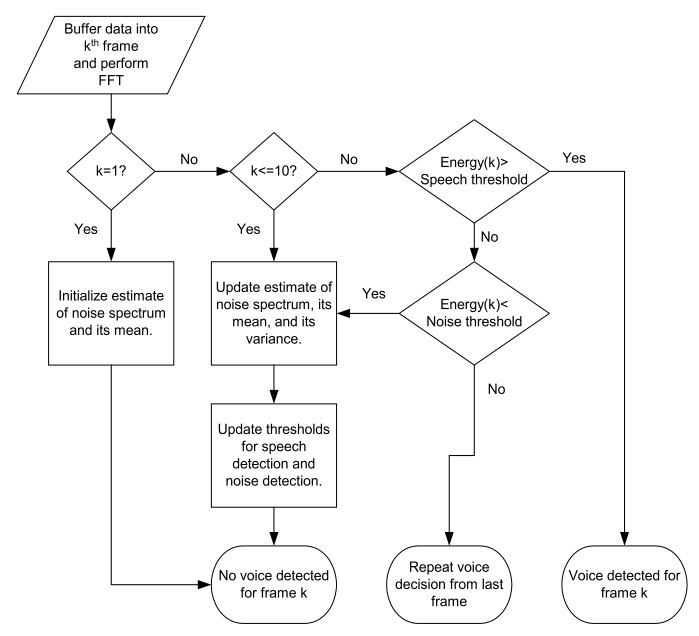
\includegraphics[width=110mm]{State_of_Art/VADener}
	\caption{VAD with energy detection\cite{Faneuff2002SpatialCar}.}
	\label{fig:VADener}
\end{figure}

Some other methods can be found in \cite{Faneuff2002SpatialCar}, \cite{Rubio2007Two-microphoneEstimates},\cite{Rosca2002MultichannelEnvironments}, \cite{Gerkmann2011NoisePresence},\cite{Nelke2013DualProbability}. Some of them are listed:

\begin{itemize}
\item Zero crossing rates: these can be calculated for each frame and compared with a threshold. The zero crossing rate of noise is assumed to be considerably larger than the one of speech. This assumption works well at high SNR values, but has problems at low SNR and in the presence of periodic noise.

\item Periodicity: The detector uses a least-squares periodicity estimator, LSPE, on the input signal and triggers when a significant amount of periodicity is found.


\item Speech Presence Probability (SPP):  it is shown \cite{Gerkmann2011NoisePresence} that it is possible to create a limited maximum likelihood estimator, then use it for the estimation of the a priori signal-to-noise ratio (SNR), and this resulting noise power estimate can be updated when the a posteriori SNR is below a certain threshold and, finally, this threshold can be seen as a voice activity detector. 


\end{itemize}

\subsection{Spectral subtraction}

This algorithm uses the short-term spectral magnitude of the noisy speech and estimate or reference of the noise signal. Most of the single channel spectral subtraction methods use a VAD to determine if there is silence or not in order to get an accurate noise estimate and the noise is assumed to be short term stationary so that noise from silence frames can be used to remove noise from voiced frames as shown in figure \ref{fig:duagSS}.


\begin{figure}[!ht]
  \center
	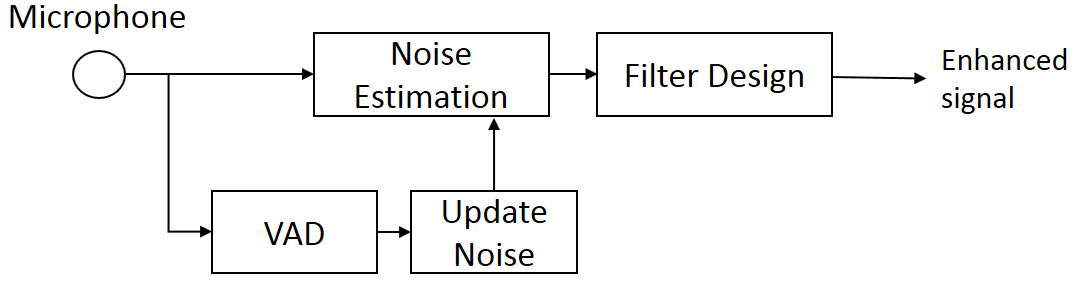
\includegraphics[width=110mm]{State_of_Art/duagSS}
	\caption{Basic Spectral Subtraction.}
	\label{fig:duagSS}
\end{figure}


Many articles show different ways of using the spectral subtraction as \cite{Ephraim1984SpeechEstimator}, \cite{MeyerSubtraction.pdf}, \cite{Smaragdis1998BlindDomain}, \cite{Abdelaziz2005Real-TimeEnhancement}.

The spectral subtraction always uses a VAD. This is used to know the noise power only in the silence periods and this information is used to erase the noise from the speech as we can see in the figure \ref{fig:scspecSubs}.

\begin{figure}[!ht]
  \center
	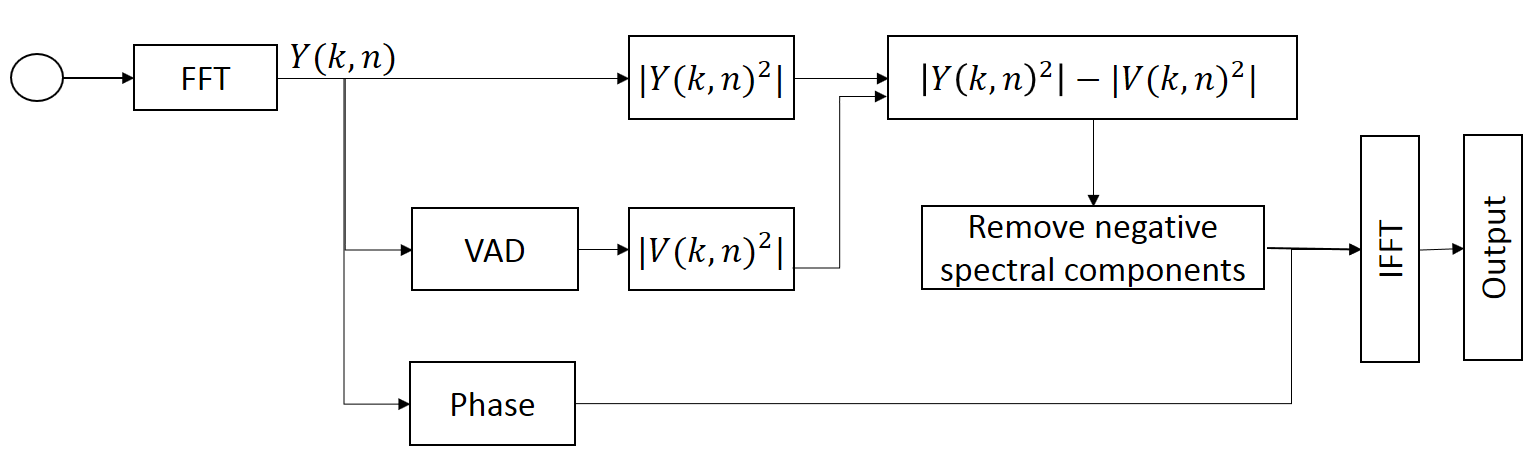
\includegraphics[width=110mm]{State_of_Art/scspecSubs}
	\caption{Single Channel Spectral Subtraction.}
	\label{fig:scspecSubs}
\end{figure}


\subsection{Talker isolation}

It is necessary to isolate the desired speech from other speech sources and noise. In this case, separating the sources is crucial since the desired and undesired speech have similar spectra and comparable amplitudes.

It is used the frequency and amplitude continuity to track the desired talker. Binaural spatial cues are used to discriminate pitch frequencies that are too close to resolve spectrally. In \cite{Luo1994AReverberation} they show an example using a combination of techniques for advanced pitch tracking and talker isolation, it is used frequency and amplitude continuity to track the desired talker.



\section{Multiple Channel Algorithms}


\subsection{Sources separation}

The separation of sources is an approach in which the source signals are estimated from the mixed signals observed in each channel. This technique is used in sound systems in order to erase noise or to erase the cross-talking in communications. This system can be modeled as seen in figure \ref{fig:sepa} (with 2 sources).


\begin{figure}[!ht]
  \center
	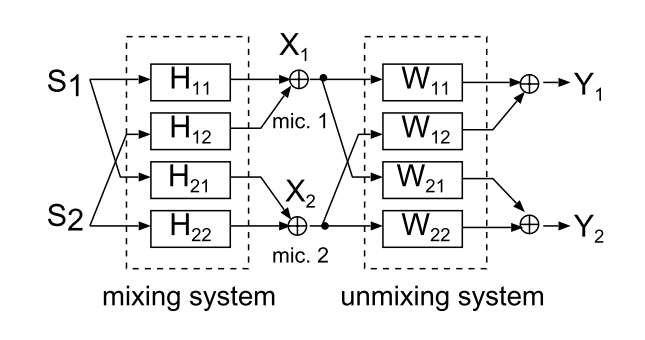
\includegraphics[width=90mm]{State_of_Art/sepa}
	\caption{Separation of sources system configuration.}
	\label{fig:sepa}
\end{figure}

Many methods have been developed to achieve a proper separation of sources. In \cite{Smaragdis1998BlindDomain} it is shown a method in which, as some other methods like \cite{Bourgeois2004Frequency-domainCorrelation} and \cite{Mei2006BlindCriterion}, every filter of the unmixing system ($W_{ij}$) is found by an estimation of the mixing system ($H_{ij}$). 



\subsection{Beamforming}

Beamforming is the term used for steering an array of sensors (microphones) to have unity gain in the direction of the desired source and attenuate the signals with origin in other directions. Source localization can be important to improve the effect of beamforming \cite{Faneuff2002SpatialCar}. This can be used as a noise reduction method due to it's capacity of localization, that means that the noise (which comes from different directions than the voice) will be attenuated. 


The technique of beamforming is used to capture multiple sound inputs $s(t)$ in the farfield and, after filtering and addition obtain a reference signal $Z$ \cite{Faneuff2002SpatialCar}. 


%\begin{figure}[!ht]
%  \center
%	\includegraphics[width=110mm]%{Kap3/bf_beam_pattern}
%	\caption{Beamforming system %configuration.}
%	\label{fig:bf_beam_pattern}
%\end{figure}


One technique called the "delay and sum beamformer" , which is probably the simplest, consist in apply a phase delay to the input signals to steer the main lobe directivity to an specific direction. 

\subsection{Coherence and Speech Presence Probability}

In \cite{Nelke2013DualProbability} is proposed one noise estimation method based in the speech presence probability value showed in \cite{Gerkmann2011NoisePresence} and the coherence function, which behaves as a measure of spectral similarity between signals. The coherence function, due to the noise characteristics of noise in diffuse field, has low values for noisy segments and a high value for speech segments.

\subsection{Multi-Channel Wiener Filter}

The Wiener filter is a filter used to produce an estimate of a desired or target, assuming known stationary signal and noise spectra, and additive noise. The goal of the this filter is to find a statistical estimate of an unknown signal using a reference signal as an input and filtering this signal to produce the estimate as an output. 
In \cite{Yong2013} it is proposed a multichannel method which also uses one single channel method as reference. This algorithm will be described in detail later since it was chosen for implementation.



\chapter{The Problem and its Background}

As it was shown in the introduction, this work pretends to prove several VAD and SPP methods for the multichannel Wiener filter algorithm for speech enhancement. In this chapter will be explained how this filter works and why it is important to test the performance of the SPP block.


\section{Signal Model}

To maintain mathematical coherence during the document, the signal model will always be as it follows:

The microphone signals will be denoted as:

$$Y_m(k,n),l=1,...,M$$

Where $k$ is the frequency bin index, $n$ is the frame index and $M$ is the number of microphones. So, the input signals are given by:

$$Y_m(k,n)=X_m(k,n)+V_m(k,n)$$

Where $X_m$ and $V_m$ are the target signal and the uncorrelated noise components. The goal is to remove the unwanted noise and preserve the target signal, this can be done by using a filter set $\textbf{w}(k,n)$ to obtain:

$$Z(k,n)=\textbf{w}^H(k,n)\textbf{y}(k,n)$$



Where $Z$ is the output signal and $\textbf{y}(k,n)$ is a vector given as:

$$\textbf{y}(k,n) = [Y_1(k,n), Y_2(k,n),...,Y_M(k,n)]^T $$
$$\textbf{y}(k,n)= \textbf{x}(k,n)+\textbf{v}(k,n)$$

The correlation matrices of noisy speech, clean speech and noise are defined as:

$$\textbf{R}_y=E\{\textbf{yy}^H\}  	\in \mathds{C}^{M\times M}$$
$$\textbf{R}_x=E\{\textbf{xx}^H\}	\in \mathds{C}^{M\times M}$$
$$\textbf{R}_v=E\{\textbf{vv}^H\}	\in \mathds{C}^{M\times M}$$



\section{Multi-Channel Wiener Filter}

Many of the real time implementations of the multichannel Wiener filter (MWF) have estimation problems caused mainly for using a voice activity detector (VAD), which may fail in adverse environments and the use of second order clean speech statistics, which usually causes overestimation errors. In this document it will be described the algorithm proposed in \cite{Yong2013}, first using the hard VAD and then using a SPP. Also, in order to have a better performance it will be chosen one of the input signals from the microphone array and will be filtered by a single channel algorithm and this new signal will be used as reference (the complete block diagram is shown in figure \ref{fig:diagMWF}). Finally it will be shown the objective tests that were applied to this algorithm in order to show a comparison with other  methods.

\begin{figure}[!ht]
  \centering
	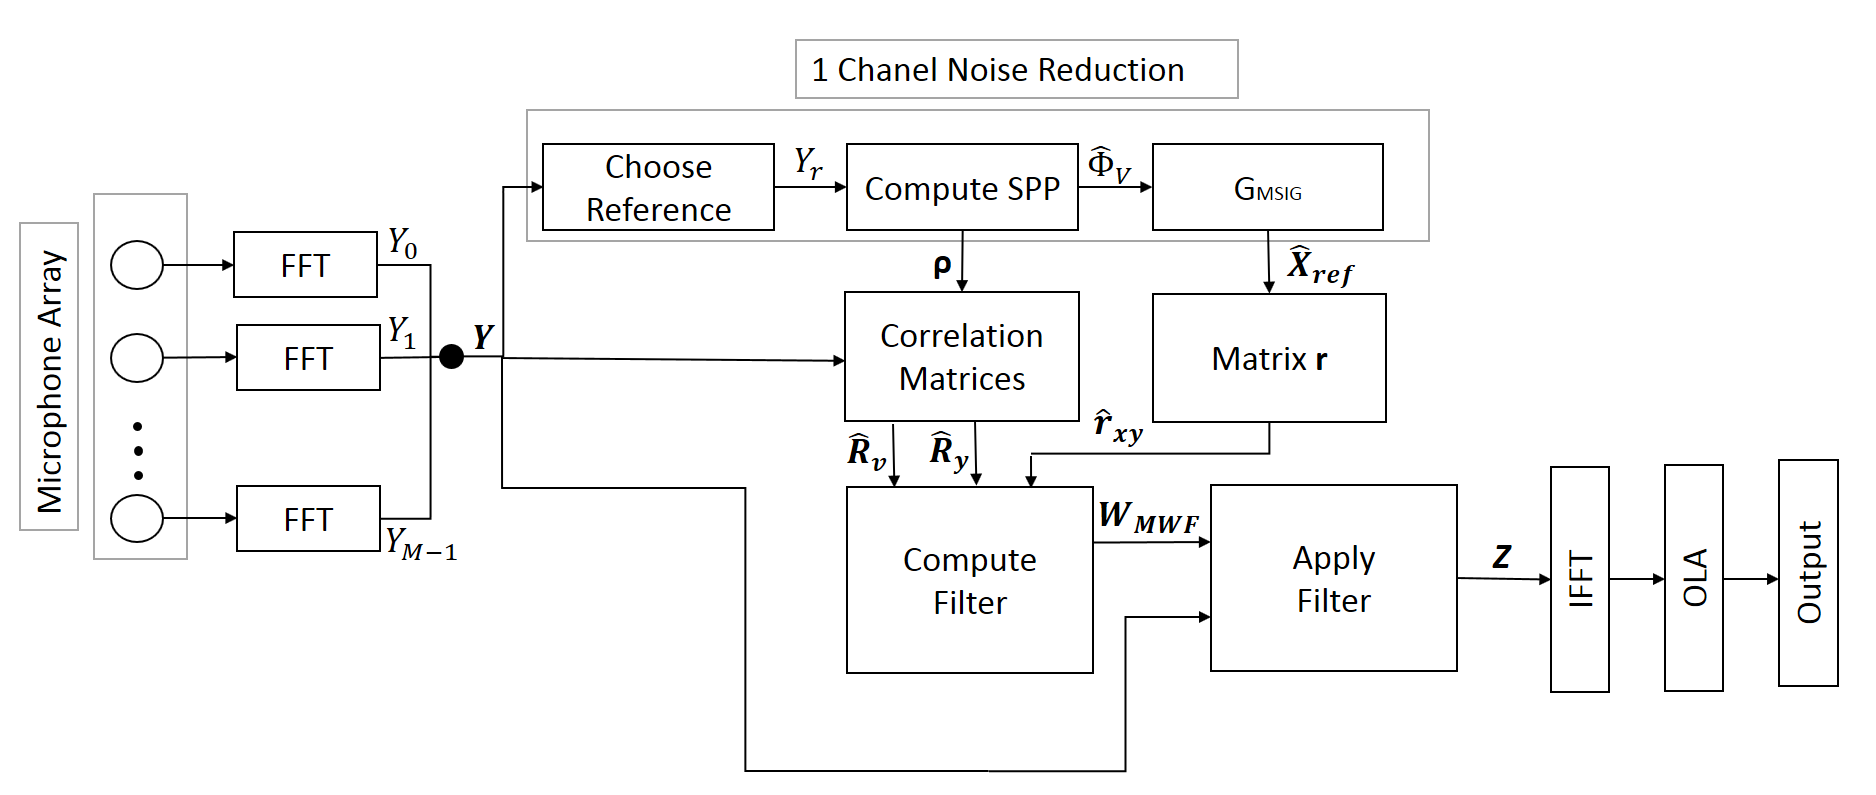
\includegraphics[width=150mm]{Kap2/diagMWF}
	\caption{Block diagram for multichannel Wiener filter.}
	\label{fig:diagMWF}
\end{figure}

\subsection{Filter Formulation}

It is expected to estimate the speech signal based on an minimum mean square error criterion as:

\begin{equation}
\textbf{w}_{MWF}=arg min_w E\{|X_{ref}-\textbf{w}^H \textbf{y}|^2 \}
\label{criteria}
\end{equation}


If it is taken the assumption of uncorrelation between speech and noise, it is possible to modify the criterion of the MWF as:

$$\textbf{w}_{MWF}=arg min_w E\{|X_{ref}-\textbf{w}^H \textbf{x}|^2 \}+\mu E\{|X_{ref}-\textbf{w}^H \textbf{v}|^2 \}$$

A larger $\mu$ value here indicates more residual noise reduction at the expense of higher speech distortion. The solution of $MWF_\mu$ can then be obtained as:

\begin{equation}
\textbf{w}_{{MWF}_\mu} = [\textbf{R}_x+\mu \textbf{R}_v]^{-1}\textbf{R}_x\textbf{e}_{ref}
\label{wiener}
\end{equation}

Where $\textbf{e}_{ref}=[0...0 1 0...0]^T$ is a M-element zero vector with the unity corresponds to the $m^{th}$ element of the microphones. 


In first place, the update of the correlation matrices can be done like:

\begin{equation}
\mathcal{H}_0 : \left\{
\begin{array}{c l}
   \hat{\textbf{R}}_v[n]=(1-\alpha_v)\hat{\textbf{R}}_v[n-1]+\alpha_v\textbf{y}[n]\textbf{y}^H[n] \\
  \hat{\textbf{R}}_y[n]= \hat{\textbf{R}}_y[n-1]
\end{array}
\right.
\end{equation}

\begin{equation}
\mathcal{H}_1 : \left\{
\begin{array}{c l}
   \hat{\textbf{R}}_y[n]=(1-\alpha_y)\hat{\textbf{R}}_y[n-1]+\alpha_y\textbf{y}[n]\textbf{y}^H[n] \\
  \hat{\textbf{R}}_v[n]= \hat{\textbf{R}}_v[n-1]
\end{array}
\right.
\end{equation}

Where  $\mathcal{H}_0$  and  $\mathcal{H}_1$ denote the periods of absence and presence of speech. This periods are determined by the use of a VAD algorithm. The choice of the smoothing factors  $\alpha$ must be done carefully taking care if the  degree of stationarity of speech and noise signals.

In equation \eqref{wiener} it is needed an estimation of $\textbf{R}_x$ which could be obtained form $\textbf{R}_y-\textbf{R}_v$, but this estimation might have some errors caused by the complex valued matrices, which will lead to a bad estimation.  This estimation could be improved by obtaining a pre-determined $R_x$ estimate  with a calibration sequence, or by implementing a mathematical model, these methods rely on the a priori information, which makes them less stable and difficult to use for final users. 

\subsection{Formulation of {$MWF_\lambda$}  and Estimation of Correlation Matrices}

To minimize the error from equation \eqref{criteria}, another criterion to minimize the noise power is proposed. For this, one weighed sum can be find as:

$$\textbf{w}_{MWF_\lambda}=argmin_w(1-\lambda)E\{|X_{ref}-\textbf{w}^H\textbf{y}|^2\}+\lambda(E\{|\textbf{w}^H\textbf{v}|^2\})$$

Where $\lambda$ is a weighting value between 0 and 1, this solution is given by:

\begin{equation}
\textbf{w}_{MWF_\lambda}=[(1-\lambda)\textbf{R}_y+\textbf{R}_v]^{-1}(1-\lambda)\textbf{r}_{yx}
\label{mwfl}
\end{equation}


$$\lambda=1-\rho$$
where $\textbf{r}_{yx}=E\{\textbf{y}X^*_{ref}\}$.   Using this consideration, it is avoided the estimation of $\textbf{R}_x$ and the value of $\lambda$ can be set as $1-\rho$ where $\rho$ is the SPP of the signal. Also,  it is proposed to avoid the decision by the VAD to estimate the correlation matrices and to use instead a modified SPP ($\rho$) with which the matrices can be estimated as:




\begin{equation}
\hat{\textbf{R}}_v[n]=(1-\tilde{\alpha}_v[n])\hat{\textbf{R}}_v[n-1]+\tilde{\alpha}_v[n]\textbf{y}[n]\textbf{y}^H[n] 
\label{corrv}
\end{equation}

\begin{equation}
\hat{\textbf{R}}_y[n]=(1-\tilde{\alpha}_y[n])\hat{\textbf{R}}_y[n-1]+\tilde{\alpha}_y[n]\textbf{y}[n]\textbf{y}^H[n]
\label{corry}
\end{equation}


Where $\tilde{\alpha}_v$ and $\tilde{\alpha}_y$  are given by:

$$\tilde{\alpha}_v=\alpha_v(1-\rho)$$ and

$$\tilde{\alpha}_y=\alpha_y\rho$$

Where $\alpha_v$ and $\alpha_y$ are the fixed smoothing factors for noise and noisy correlation matrices and $\rho$ is the value of the speech presence probability. 


\subsubsection{Smoothing the filter}

In the first implementation, as proposed in \cite{Yong2013}, the output signal tends to have musical noises. To solve this, it is proposed to do a smoothing process over the whole filter $\textbf{W}_{MWF_\lambda}$ as:

\begin{equation}
 \textbf{W}_{MWF_\lambda}(k,n)= \alpha_w\textbf{W}_{MWF_\lambda}(k,n-1)+(1-\alpha_w) [(1-\lambda)\textbf{R}_y+\textbf{R}_v]^{-1}(1-\lambda)\textbf{r}_{yx}
\label{mwfeq}
\end{equation}


Which leads to an important musical noise reduction.

\subsubsection{Single-Channel Reference}

From equation \eqref{mwfl}, we can see that this method needs the estimate of the speech reference $X_{ref}$, to achieve this, it is proposed to estimate $X_{ref}$ by using a single-channel speech enhancement method and to use one microphone as a reference. With this, it is possible to define: $$\tilde{\textbf{r}}_{yx}=\textbf{y}G(X^*_{ref}+V^*_r)$$

Where $X_{ref}=H_{ref}S$, in which $H_{ref}$ is the acoustic transfer function of the target speech signal $S$, at the reference channel. In this equation $G$ is a spectral weighting gain function, which involves the computation of the \textit{a posteriori }and \textit{a priori} SNR estimates. Also, to avoid musical noise, it is proposed to update recursively $\hat{\textbf{r}}_{yx}(n)$ as:

\begin{equation}
\hat{\textbf{r}}_{yx}(n)=(1-\alpha_x)\hat{\textbf{r}}_{yx}(n-1)+\alpha_x\textbf{y}(n)\hat{X}^*_{ref}(n)
\label{requ}
\end{equation}


Where $\alpha_x$ is the smoothing  factor for target speech signal, and $\hat{X}_{ref} = G(X_{ref}+V_r)$  indicates the clean speech estimate from the reference microphone.  This estimate  can be done with any of the existent speech enhancement methods, but it is recommended to use one in which the  speech distortion can be controlled and set it as small as possible. In this case it will be used the one found in \cite{Yong2013OptimizationEnhancement}. This method works as follows:   

\subsubsection{Sigmoid function with \textit{a priori} SNR}



In order to find $\hat{X}_{ref}$ it is needed to chose one of the channels as a reference, in our case the input  of the closest microphone to the source can be chosen. This signal must be filtered with one method of speech enhancement. 


In \cite{Yong2013OptimizationEnhancement} it is proposed to use a gain function which can be easily controlled and that has a flexible shape.   In this case we use the modified sigmoid gain function:

\begin{equation}
G_{MSIG}(k,n)=\frac{1-exp[-a_1 \hat{\xi}(k,n)]}{1+exp[-a_1 \hat{\xi}(k,n)]}*\frac{1}{1+exp(-a_2 [\hat{\xi}(k,n)-c])}
\label{gainSig}
\end{equation}

Where $\xi$ is the  \textit{a priori} SNR  defined as 
$$\xi(k,n)=\frac{\Phi_x(k,n)}{\Phi_v(k,n)}$$

Which can be estimated as a function of the \textit{a posteriori} SNR and an instantaneous \textit{a priori} SNR, the \textit{a posteriori} SNR and applying a recursive smoothing procedure:

$$\xi_{inst}(k,n)=max\{\gamma(k,n)-1,0\}$$

using the fact that $X(k,n-1)=G_{MSIG}(k,n)Y(k,n-1)$:

$$\hat{\xi}(k,n)=\alpha_{SNR}G_{MSIG}^2(k,n-1)\gamma(k,n-1)+(1-\alpha_{SNR})\xi_{inst}(k,n) $$
The variance in the\textit{ a priori} SNR estimate can lead to audible musical noise due to the higher sensitivity to changes. In order to reduce such musical noise, a first order recursive smoothing procedure, as shown in \cite{Yong2011OnEnhancement}, can be applied in the \textit{a posteriori }SNR estimation:

$$\bar{\gamma}(k,n)=\frac{\Phi_y(k,n)}{\hat{\Phi}_v(k,n)}$$
With:

$$\Phi_y(k,n)=\alpha_{y'}\Phi_y(k,n-1)+(1-\alpha_{y'})|Y(k,n)|^2$$



The resulting function of equation \eqref{gainSig}  can have different shapes as shown in \ref{fig:sigm} according to the choice of the constants $a_1$, $a_2$ and $c$, for this implementation the values were chosen as function MSIG-fix3:

$$a_1=15$$
$$a_2     = 0.6351$$
$$c       = 0.2243$$
\begin{figure}[!ht]
  \centering
	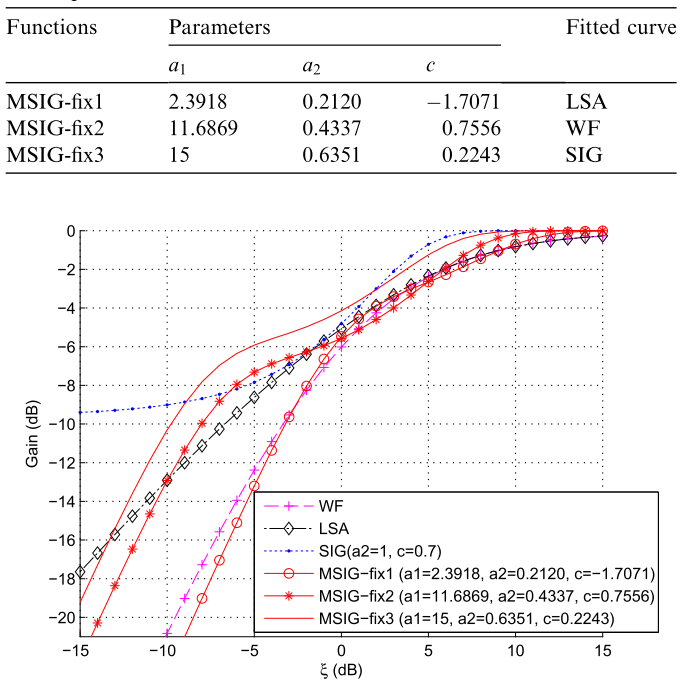
\includegraphics[width=110mm]{Kap2/sigm}
	\caption{Different shapes of the gain function, taken from \cite{Yong2013OptimizationEnhancement}.}
	\label{fig:sigm}
\end{figure}



\section{Speech Presence Probability}

Several authors have made important research on SPP methods. 

All real time audio processing algorithms are implemented with short time Fourier transformations (STFT). The speech presence probability method, has as output a vector of the same size than each frame vector, each element of this vector is a real number with values from 0 to 1 which denote the probability of finding voice in each frequency bin. In this case 0 is the lowest probability of finding voice and 1 is the highest. In the figure \ref{fig:spectro} it is shown the spectrogram of a clean female voice signal and in figure \ref{fig:SPP} it is shown all the SPP vectors of this signal. 

\begin{figure}[!ht]
  \centering
	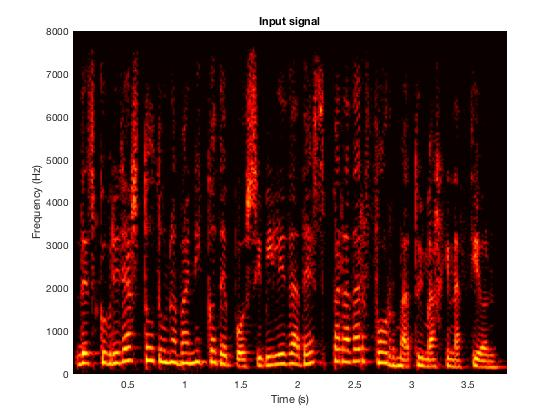
\includegraphics[width=100mm]{Kap2/spectro}
	\caption{Spectrogram of a clean voice audio file.}
	\label{fig:spectro}
\end{figure}

It is possible to see that, in an ideal SPP (absence of noise), the output has the value of 1 in each bin where there is presence of speech in the signal. Note that in an ideal case all speech presence values should be 1 and this does not depend on the magnitude of the voice energy in the signal, following the same logic, in silent segments or nose segments, the values should be 0. 

\begin{figure}[!ht]
  \centering
	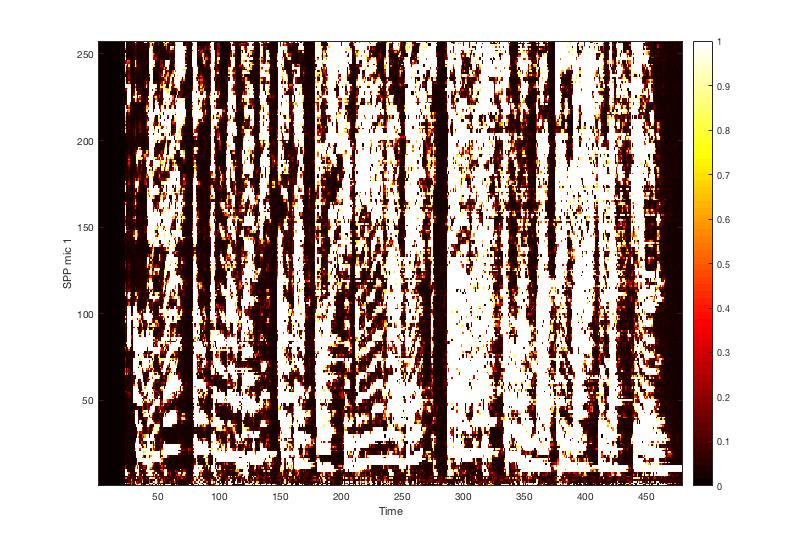
\includegraphics[width=100mm]{Kap2/SPP}
	\caption{Speech presence probability of a clean voice audio file.}
	\label{fig:SPP}
\end{figure}

In this project, different algorithms for finding the SPP will be tested under different SNR conditions. For testing this, the SNR of the output of the MWF will be compared for each SPP algorithm.


\chapter{Speech Presence Probability Implementation}

In this chapter it will be shown how the SPP method found in \cite{Gerkmann2011NoisePresence} can be implemented in Matlab so that the different variations in the algorithm can be tested later.

\begin{figure}[!ht]
  \centering
	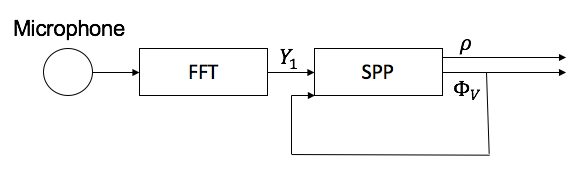
\includegraphics[width=100mm]{Kap3/SPPdiag}
	\caption{Block diagram of SPP method.}
	\label{fig:SPPdiag}
\end{figure}

\section{Implementation}

Under the assumption that a soft decision VAD might be more precise than the hard decision, the following algorithm will be included in the  multi-channel noise reduction method.  Following this, the SPP was found as proposed in \cite{Gerkmann2011NoisePresence}: 

\begin{equation}\label{SPP}
{\rho=\frac{1}{\left( 1+(1+\xi_{opt})exp\left(-\frac{|Y_1(k,n)|^2}{\Phi_{V}(k,n-1)}\frac{\xi_{opt}}{\xi_{opt}+1}\right)\right)}}
\end{equation}


Where $\rho$ is the variable that takes values between 0 and 1 indicating the probability of voice presence (0 means no voice, 1 means total certitude of voice) and  $\xi_{opt}$ is a fixed a priori SNR, $Y_1$ is the input , $\Phi_V$ is the noise power density, and:

\begin{equation}
\Phi_{V,SPP}(k,n)=\rho \Phi_{V,SPP}(k,n-1)+(1-\rho)|Y_1(k,n)|^2
\label{psdNoi}
\end{equation}


After this, the value of $\Phi_{N,SPP}$ is integrated to the estimated noise power density:

\begin{equation}
\Phi_{V}(k,n)=\alpha_{N,SPP} \Phi_{V}(k,n-1)+(1-\alpha_{N,SPP})\Phi_{V,SPP}(k,n)
\label{noipsdc}
\end{equation}

In \cite{PeiCheeYongSvenNordholm2012NoiseSmoothong} it is proposed a similar method in which the value of $\rho$ is modeled as a sigmoid function, with this, it is possible to adjust its slope ($a_{sig}$)  and mean ($c_{sig}$). The value of $\rho$ wil be given as:

\begin{equation}\label{SPPyong}
{\rho=\frac{1}{\left( 1+exp\left(-a_{sig}\left(\frac{|Y_1(k,n)|^2}{\Phi_{V}(k,n-1)}-c_{sig}\right)\right)\right)}}
\end{equation}


where:

$$a_{sig}=\frac{\xi_{opt}}{\xi_{opt}+1}$$
$$c_{sig}=log\left(\frac{P(\mathpzc{H}_0)}{P(\mathpzc{H}_1}(1-\xi_{opt}) \right)\frac{\xi_{opt}+1}{\xi_{opt}}$$

In this project both SPP methods will be tested and compared when they are used with as part of the MWF noise reduction method.

\section{Stagnation}

This algorithms give a very close estimation of the ideal SPP, but, it is susceptible to have stagnation problems. It can be seen that if the spectral noise power is underestimated, in equation \eqref{SPP}, it may lead to $\rho=1$ even if the power of the input is low with respect to the real and unknown noise power. In this case the equation \eqref{psdNoi} won't update the noise power anymore and the noise will remain underestimated. This is know as stagnation.

Both described  methods also propose a way to avoid stagnation which will be explained in this chapter and part of the testing algorithms.

\subsubsection{Tracking Time Average}

The algorithm showed in \cite{Gerkmann2011NoisePresence} propose to force a lower the value of $\rho$ when it's time average is higher than certain threshold. This means, if $\rho$ has high values for too long it's forced to a lower one, this can be expressed as:


\begin{equation}\label{Stag1}
\rho = \left\{
\begin{array}{c l}
 min(0.5 , \rho) &  \bar{\rho}>0.9\\
 \rho & else
\end{array}
\right.
\end{equation}

\subsubsection{3 Regions}

In \cite{PeiCheeYongSvenNordholm2012NoiseSmoothong}, the SPP was categorized in three regions which control the update speed of the noise PSD  estimate from equation \ref{noipsdc} as follows:
 
\begin{equation}\label{Stag2}
\tau= \left\{ \begin{array}{lcc}
             \mathpzc{P}_1 &   if  & \rho \leq 0.3 \\
             \\ \mathpzc{P}_2 &  if & 0.3 < \rho < 0.6 \\
             \\ min(\mathpzc{P}_3,\rho) &  if  &\rho \geq 0.6
             \end{array}
   \right.
\end{equation}
 \medskip
 
 After, finding the right $\tau$, the smoothing value $\alpha$ is found with the following equation:
 
\begin{equation}
C(\tau_m)=\alpha =  e^{\frac{-2.2R}{F_{s}*\tau}}
\label{fromTime}
\end{equation}


The proposed time values for $\mathpzc{P}_i$ are:

$$\mathpzc{P}_1=50ms$$
$$\mathpzc{P}_2=80ms$$
$$\mathpzc{P}_3=240ms$$








\chapter{Evaluation}
 In this chapter it is shown the steps for implementing the MFW, the evaluation score that will be use for testing it and the results of testing it under different conditions.
 
 \section{Algorithm}
 
The MWF noise reduction method was implemented in Matlab following these steps:

\begin{enumerate}
\item Compute the auto and cross $PSD$ of both inputs.
\item Find the single microphone SPP $\rho$ and noise PSD with \eqref{SPP} or \eqref{SPPyong} and \eqref{psdNoi}
\item Apply a single channel noise reduction method to the reference. 
\item Obtain correlation matrices with \eqref{corrv} and \eqref{corry}.
\item Obtain the estimated matrix $\hat{\textbf{r}}_{yx}$ with \eqref{requ} using the filtered reference of step 3.
\item Obtain filter  $\textbf{W}_{MWF_\lambda}$  with \eqref{mwfeq}.
\item Obtain $Z$ as $Z(k,n)=\textbf{W}_{MWF_\lambda}^H(k,n)\textbf{y}(k,n)$.
\end{enumerate}

The MWF was implemented in Matlab with both previously showed SPP algorithms and with both methods to avoid stagnation. Here it will be shown how to evaluate the performance of this implementation and the results of it.

\section{Data Base}

To test in the most accurately possible way all the noise reduction methods, it is necessary to have a proper data base and a proper algorithm to run the measurement metric. For this is was used a radio studio with 4 microphones, one main speaker and a set of several speakers.

The data base consists of 10 voices (5 female and 5 male) and 5 different kind of usual noises.

The main speaker and microphones were arranged as shown in figure \ref{fig:DataB} where $D=50cm$ and $d=10cm$. The main speaker was reproducing the clean voice files and the set of speakers was placed all around the studio to create a good simulation of  spatially homogeneous distributed noise.



\begin{figure}[!ht]
  \centering
	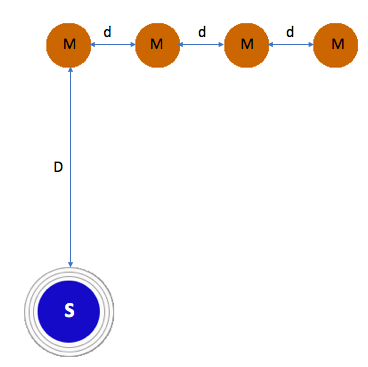
\includegraphics[width=120mm]{Kap4/DataB}
	\caption{Microphone array and audio source positions.}
	\label{fig:DataB}
\end{figure}

\section{Perceptual Evaluation of Speech Quality}

As shown in \cite{Sharma2014AMeasure}, the measure of PESQ (Perceptual Evaluation of Speech Quality) is a measure which evaluates the similarity between two speech signals in a perceptual scale. This means that a high value of PESQ means a good speech enhancement method.

The score of PESQ is given in dBs, where the higher score means better speech enhancement.

The Matlab code capable of performing the PESQ evaluation between two signals was taken from \cite{Loizou}. 

In order to obtain accurate scores, two files from the voice data base were taken (one female voice and one male voice) and two from the noise database and each voice was mixed with each noise in a range of SNR of $[-30dB , 15dB]$. These signals were taken as imputs for the different filters, and then the output of each filter was plotted and compared with the other methods and with the original noisy signal. 


\section{Results}

The results of the evaluation process are shown in figures \ref{fig:female3n}, \ref{fig:male3N}, \ref{fig:female2n}, \ref{fig:MaleN1}. The method labeled as "Gerk" refers to the one found in \cite{Gerkmann2011NoisePresence} and the one labeled as "Yong" refers to the one found in \cite{SPPYONG} and the label "Noisy" is the noisy input with no filter. The use of these methods with each of the algorithms to avoid stagnation and their combination were plotted and their PESQ score is displayed. \\






\begin{figure}[!ht]
  \centering
	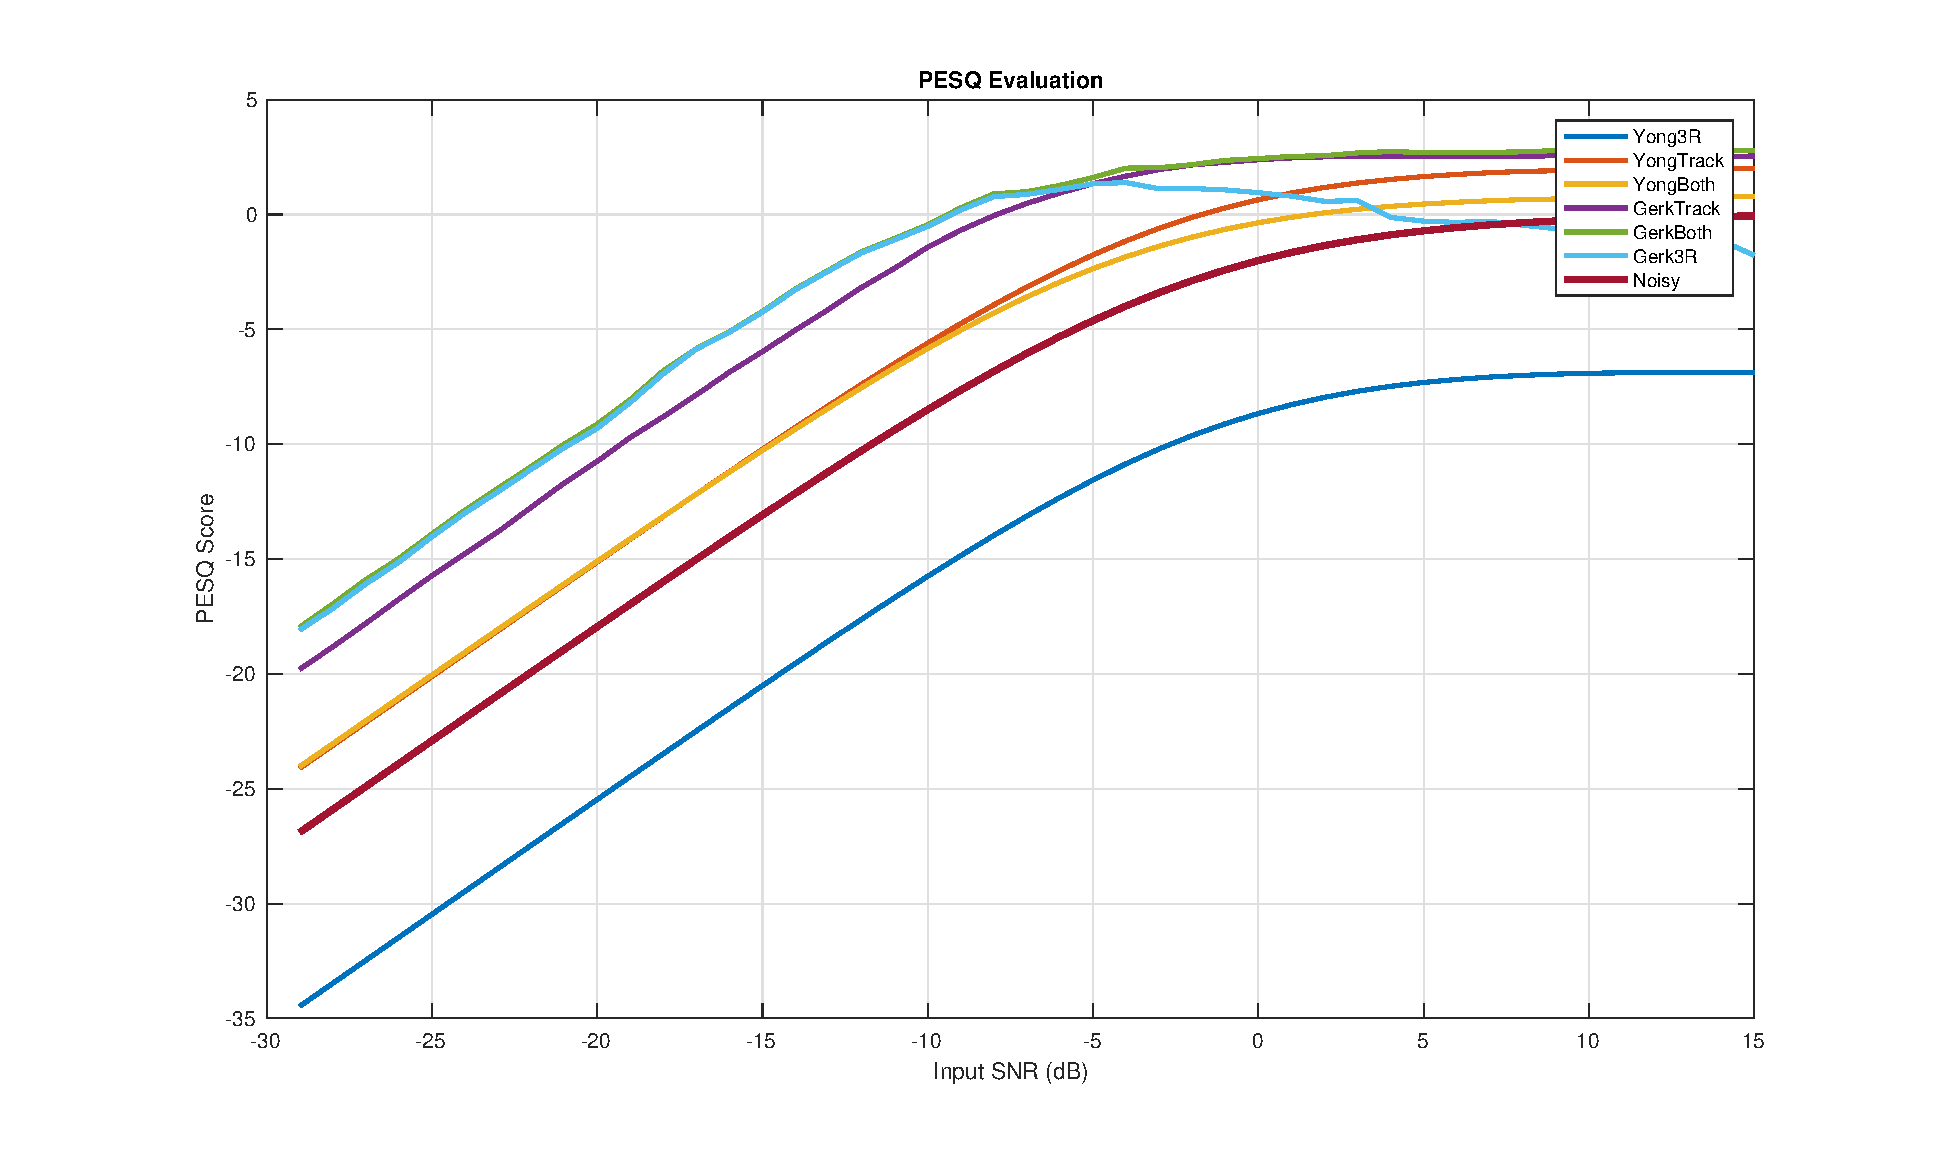
\includegraphics[width=130mm]{Kap4/female3n}
	\caption{PESQ results for female voice and car noise audios.}
	\label{fig:female3n}
\end{figure}

It can be seen in all figures that the combination of "Yong" with the 3 regions method leads to an important voice degradation and its PESQ values are always lower than the noisy input, however when this method is used with the tracking time algorithm, the score increases and there is speech enhancement. This can be caused by the speed in which this method updates the SPP value not being compatible with the 3 regions. In this case, combining both algorithms for avoiding stagnation doesn't improve the value. \\

\begin{figure}[!ht]
  \centering
	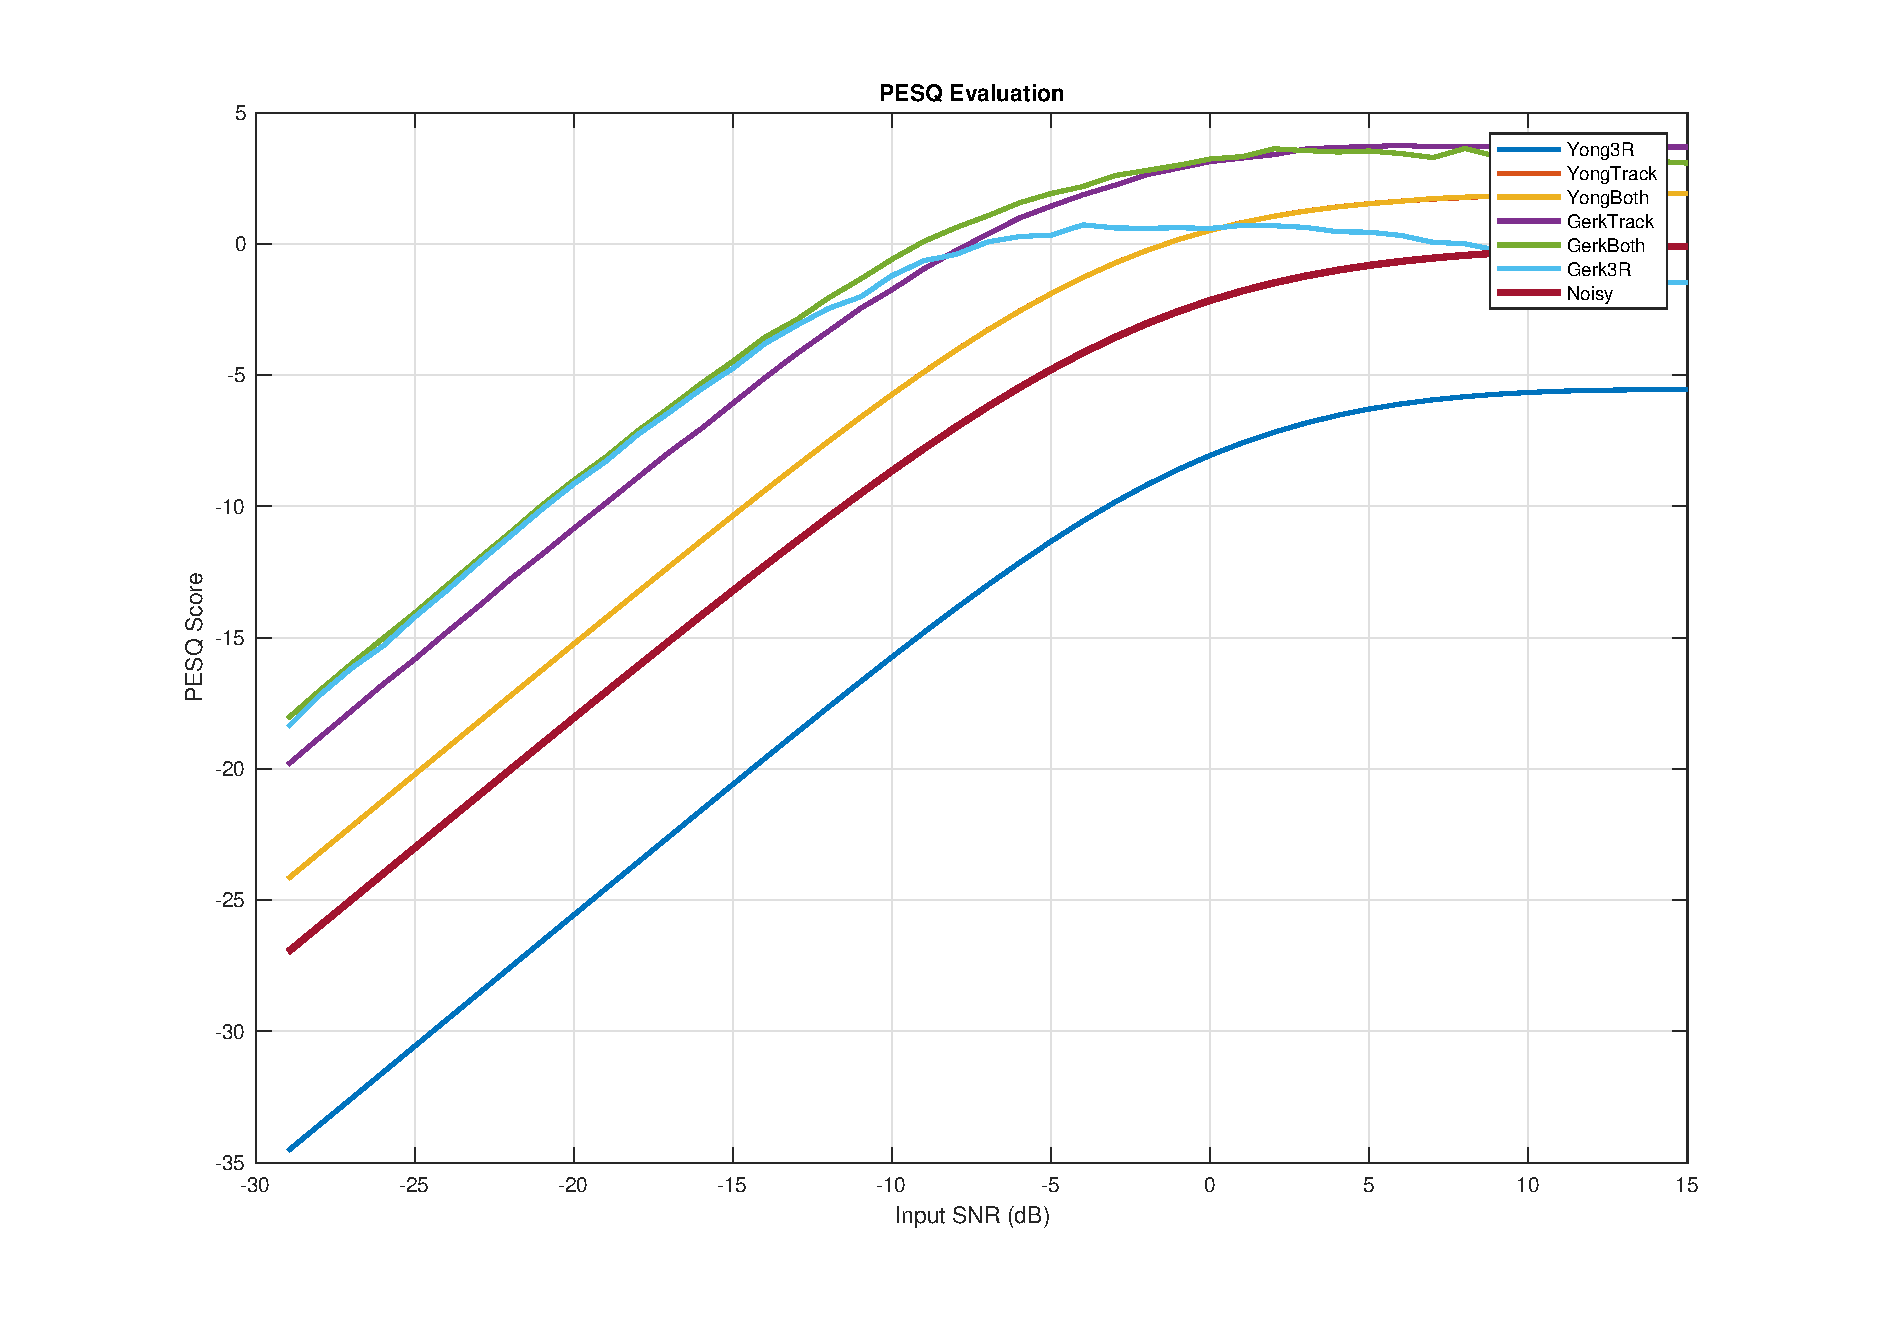
\includegraphics[width=130mm]{Kap4/male3N}
	\caption{PESQ results for male voice and car noise audios.}
	\label{fig:male3N}
\end{figure}


\begin{figure}[!ht]
  \centering
	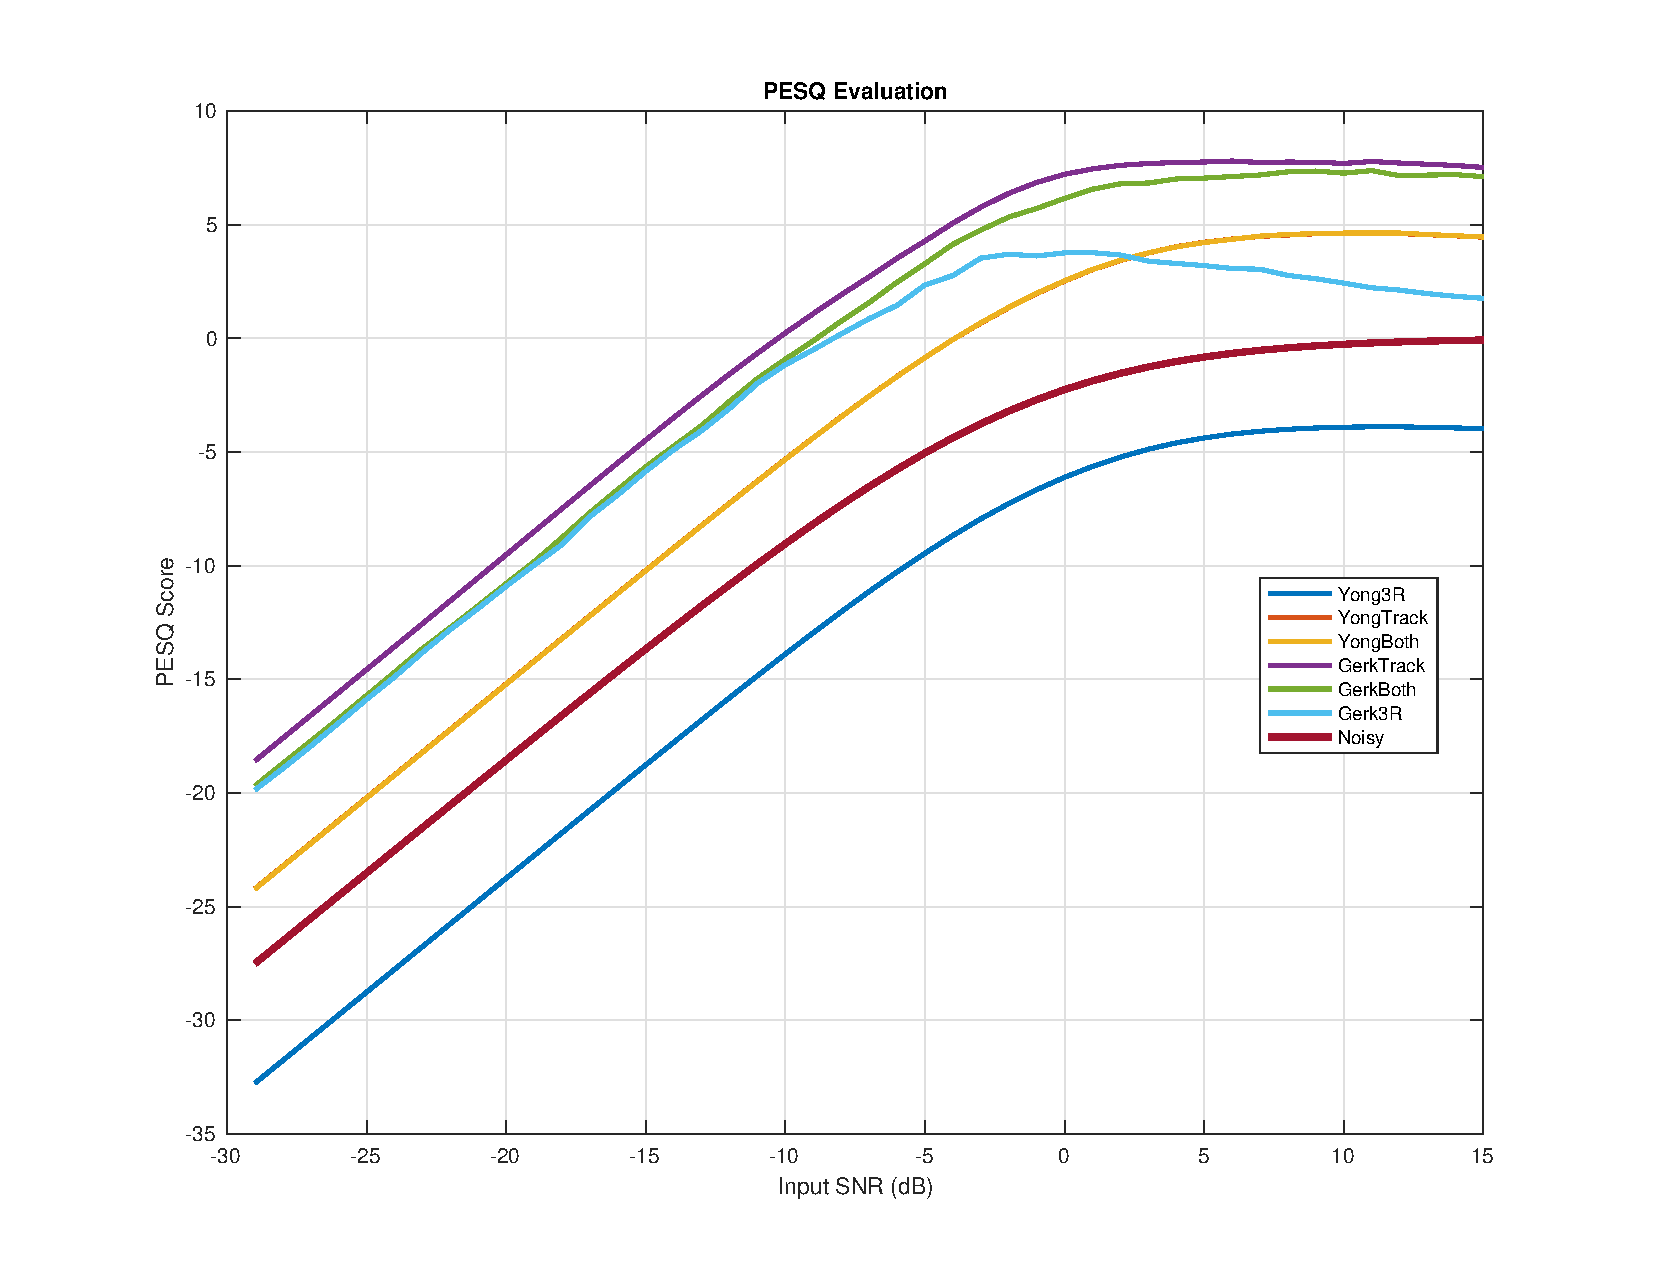
\includegraphics[width=130mm]{Kap4/female2n}
	\caption{PESQ results for female voice and street noise audios.}
	\label{fig:female2n}
\end{figure}

It can also be seen that when the method "Gerk" is combined with the 3 regions algorithm, the performance for low SNR values is always enhancing the speech but when the SNR gets higher, the scores decreases because of speech degradation. The tracking time method can help to fix this, it is shown that this method has high PESQ values for high SNR input values also when mixed with the 3 regions method.\\



\begin{figure}[!ht]
  \centering
	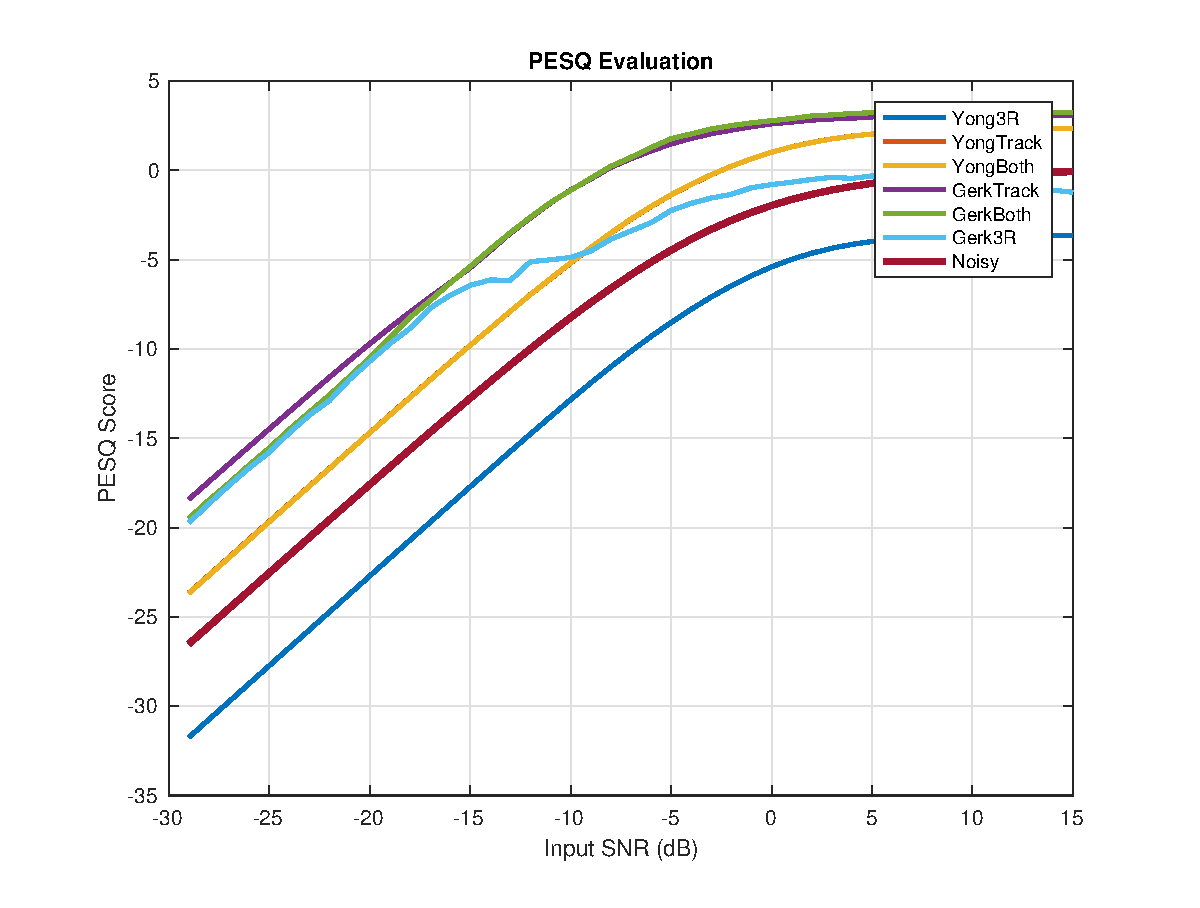
\includegraphics[width=130mm]{Kap4/MaleN1}
	\caption{PESQ results for male voice and street noise audios.}
	\label{fig:MaleN1}
\end{figure}

In general, the method shown in \cite{Gerkmann2011NoisePresence} shows a better performance when being implemented with the MWF. Also it can be noticed that the 3 regions method tends to have better performance for low SNR input values over the tracking time method but this is reversed for higher SNR values. In general, mixing these two algorithms for avoiding stagnation leads to good speech enhancement results. It is just important to notice that the tracking method will have more memory storage.\\

\begin{figure}[!ht]
  \centering
	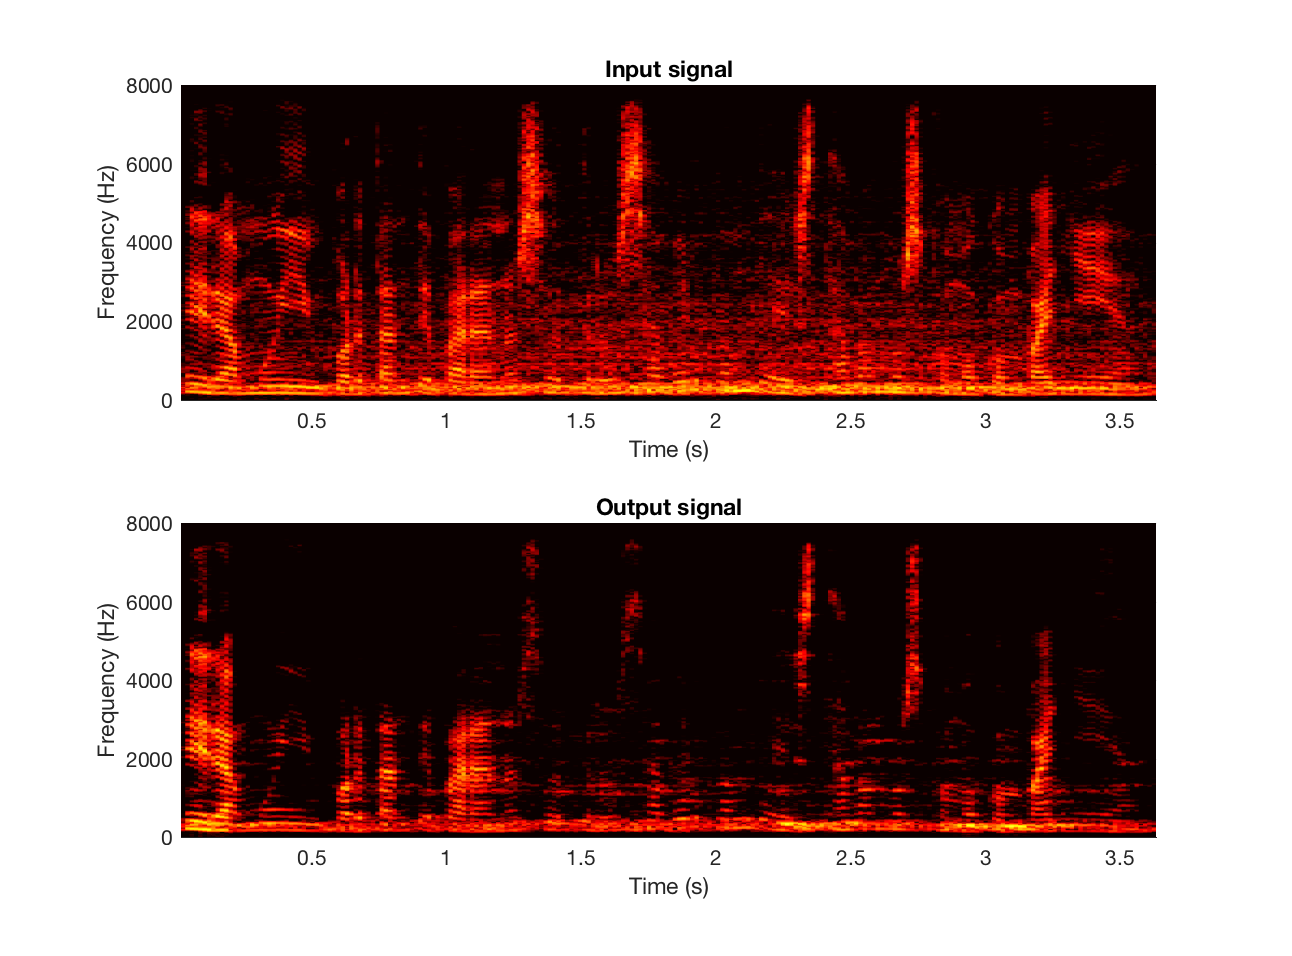
\includegraphics[width=140mm]{Kap4/fil1}
	\caption{Input and out spectrograms when using the MWF with "Gerk" method and both algorithms for avoiding stagnation.}
	\label{fig:fil1}
\end{figure}

In the figure \ref{fig:fil1} is shown the input and output spectogram of one of the test. There it is notorious how big part of the noise is attenuated while preserving the voice. In figure \ref{fig:SPP32} the SPP values of this case are show, it is notorious that there is voice over-estimation (noise taken as voice), but not under-estimation (most of the voice is detected), which is one of the conditions for having a correct reference for the multichannel filter.\\

\begin{figure}[!ht]
  \centering
	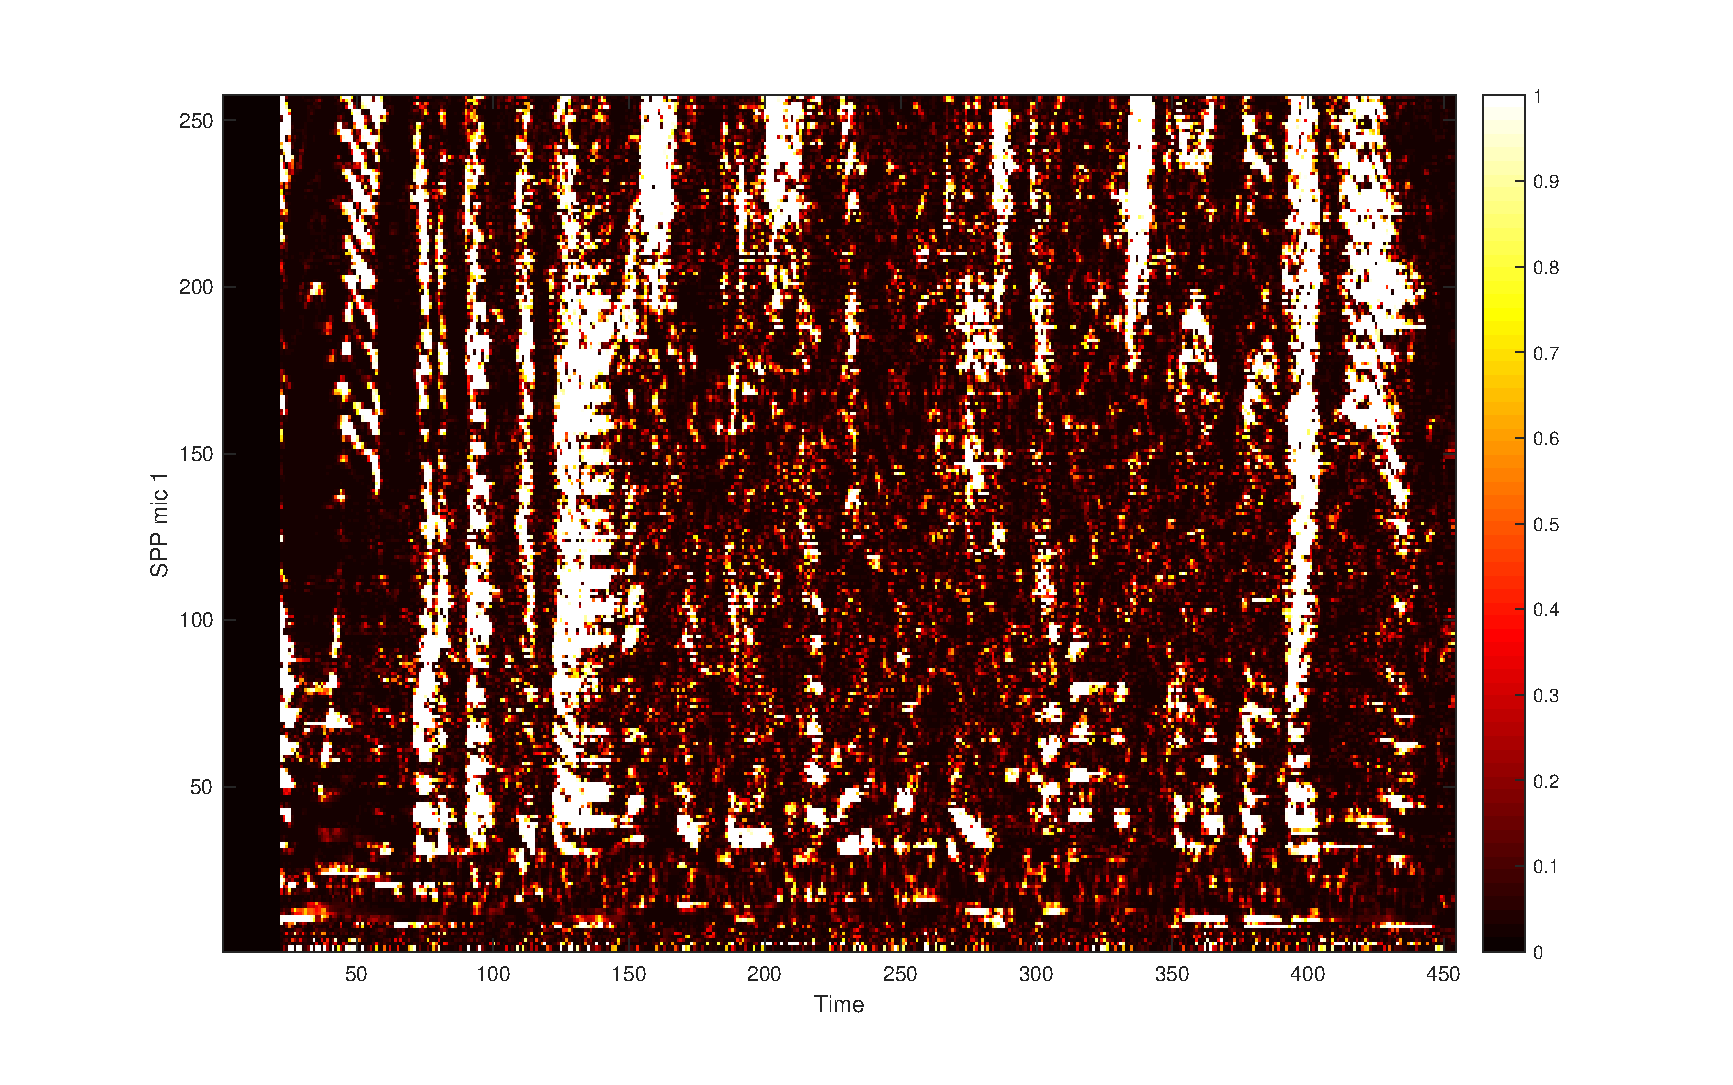
\includegraphics[width=120mm]{Kap4/SPP32}
	\caption{SPP values.}
	\label{fig:SPP32}
\end{figure}






\chapter{Conclusions and Recommendations}

\section{Conclusions}

In this document it was presented a detailed illustration of the Multichannel Wiener Filter as well as a description of each of it's blocks and how to implement them. Special attention was given to the Speech Presence Probability block and different algorithms for it were tested. The overall result shows that the method proposed in \cite{Gerkmann2011NoisePresence} when tracking time average and with the 3 regions method for avoiding stagnation.\\

The method proposed in \cite{SPPYONG} showed that is not compatible with the 3 regions method and the result of this was a lower PESQ score than the noisy input, which means that was only degrading the voice. However, when used with the tracking time average method, the results were better, but still worst that \cite{Gerkmann2011NoisePresence}.\\

The only consideration that may be done at the moment of choosing an algorithm for avoiding stagnation for \cite{Gerkmann2011NoisePresence} is that the time tracking average needs more storage memory due to it's need to save the complete vector of the smoothed SPP for every frame, which could lead to higher costs depending the implementation.




\section{Recommendations}

This complete document can be used a guide for future projects, here it can be found step by step how to implement a multichannel noise filter, a single channel noise filter, two speech presence probability methods with two different algorithms for avoiding stagnation and references on how to test any speech enhancement method. All of this can save important time for further research. \\

Also, because of the big amount of blocks that this method has, it is always possible to try to find optimum values for different situations. In the future, values like the a priori SNR and smoothing times can be tested and arranged for more specific situations.\\

These kind of algorithms is be important for communications systems and this document can be used as help for coding speech enhancement projects in mobile phones, car hands-free systems, computers, microphone arrays for public speeches and many others. \\

Finally, the data base and the code are open to be used for tests. 


















\bibliographystyle{plaindin}
\bibliography{Mendeley}
\end{document}